\documentclass[tikz, border=8pt]{standalone}
\usepackage{tikz}
\usetikzlibrary{arrows.meta, calc}

\begin{document}
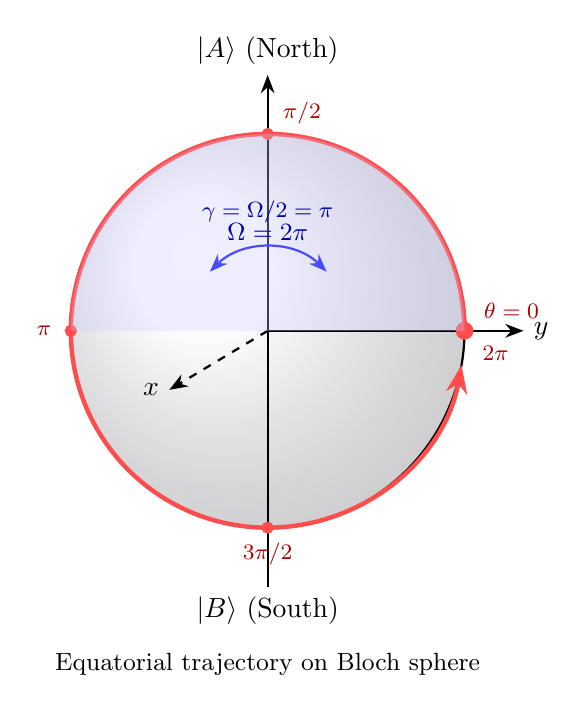
\begin{tikzpicture}[scale=2.5, >=Stealth]
    \shade[ball color=blue!5, opacity=0.3] (0,0) circle (1cm);
    \draw[thick] (0,0) circle (1cm);
    \draw[thick, ->] (0,0) -- (0,1.3) node[above] {$|A\rangle$ (North)};
    \draw[thick] (0,0) -- (0,-1.3) node[below] {$|B\rangle$ (South)};
    \draw[thick, ->] (0,0) -- (1.3,0) node[right] {$y$};
    \draw[thick, dashed, ->] (0,0) -- (-0.5,-0.3) node[left] {$x$};
    \draw[red!70, ultra thick, ->] (1,0) arc (0:350:1cm);
    \draw[red!70, ultra thick] (1,0) arc (0:10:1cm);
    \filldraw[red!70] (1, 0) circle (0.8pt);
    \node[right, font=\footnotesize, red!70!black] at (1.05, 0.1) {$\theta=0$};
    \filldraw[red!70] (0, 1) circle (0.8pt);
    \node[above right, font=\footnotesize, red!70!black, xshift=2pt] at (0, 1) {$\pi/2$};
    \filldraw[red!70] (-1, 0) circle (0.8pt);
    \node[left, font=\footnotesize, red!70!black] at (-1.05, 0) {$\pi$};
    \filldraw[red!70] (0, -1) circle (0.8pt);
    \node[below, font=\footnotesize, red!70!black, yshift=-2pt] at (0, -1) {$3\pi/2$};
    \filldraw[red!70] (1, 0) circle (1.2pt);
    \node[below right, font=\footnotesize, red!70!black, xshift=3pt, yshift=-2pt] at (1, 0) {$2\pi$};
    \fill[blue!20, opacity=0.3] (0,0) -- (1,0) arc (0:180:1cm) -- cycle;
    \node[font=\small, blue!70!black] at (0, 0.5) {$\Omega = 2\pi$};
    \draw[<->, thick, blue!70] (0.3, 0.3) arc (45:135:0.42cm);
    \node[above, font=\footnotesize, blue!70!black] at (0, 0.5) {$\gamma = \Omega/2 = \pi$};
    \node[font=\small, anchor=south] at (0, -1.8) {Equatorial trajectory on Bloch sphere};
\end{tikzpicture}
\end{document}